\documentclass[a4paper,12pt]{scrartcl}
\usepackage[utf8]{inputenc}
\usepackage[ngerman]{babel}
\usepackage{graphicx}

% Title Page
\title{Zwischenbericht Master-Projekt Bildverarbeitung}
\subtitle{SoSe 2015}
\author{Dorothee Geiser, Niels Porsiel}
\date{\today}


\begin{document}

\maketitle
\thispagestyle{empty}
\vspace{0.3\textheight}

\begin{abstract}
Im laufe des Semesters haben wir uns mit Scale-Invariant Feature Transform (kurz SIFT)
beschäftigt. Dabei haben wir uns am Paper \textit{Distinctive Image Features from Scale-
Invariant Keypoints} von David G. Lowe \cite{Lowe} orientiert. Unsere Aufgabe war es zu versuchen, 
SIFT nachzubauen. Dieser Zwischenbericht soll nun einen Überblick darüber geben, was wir 
geschafft haben.
\end{abstract}

\newpage

\section{Keypoint-Erkennung}
Dazu gehört Bild \ref{Bild1}.

\begin{figure}[htbp]
  \centering
  \includegraphics[width=0.45\textwidth]{bild}
  \fbox{ 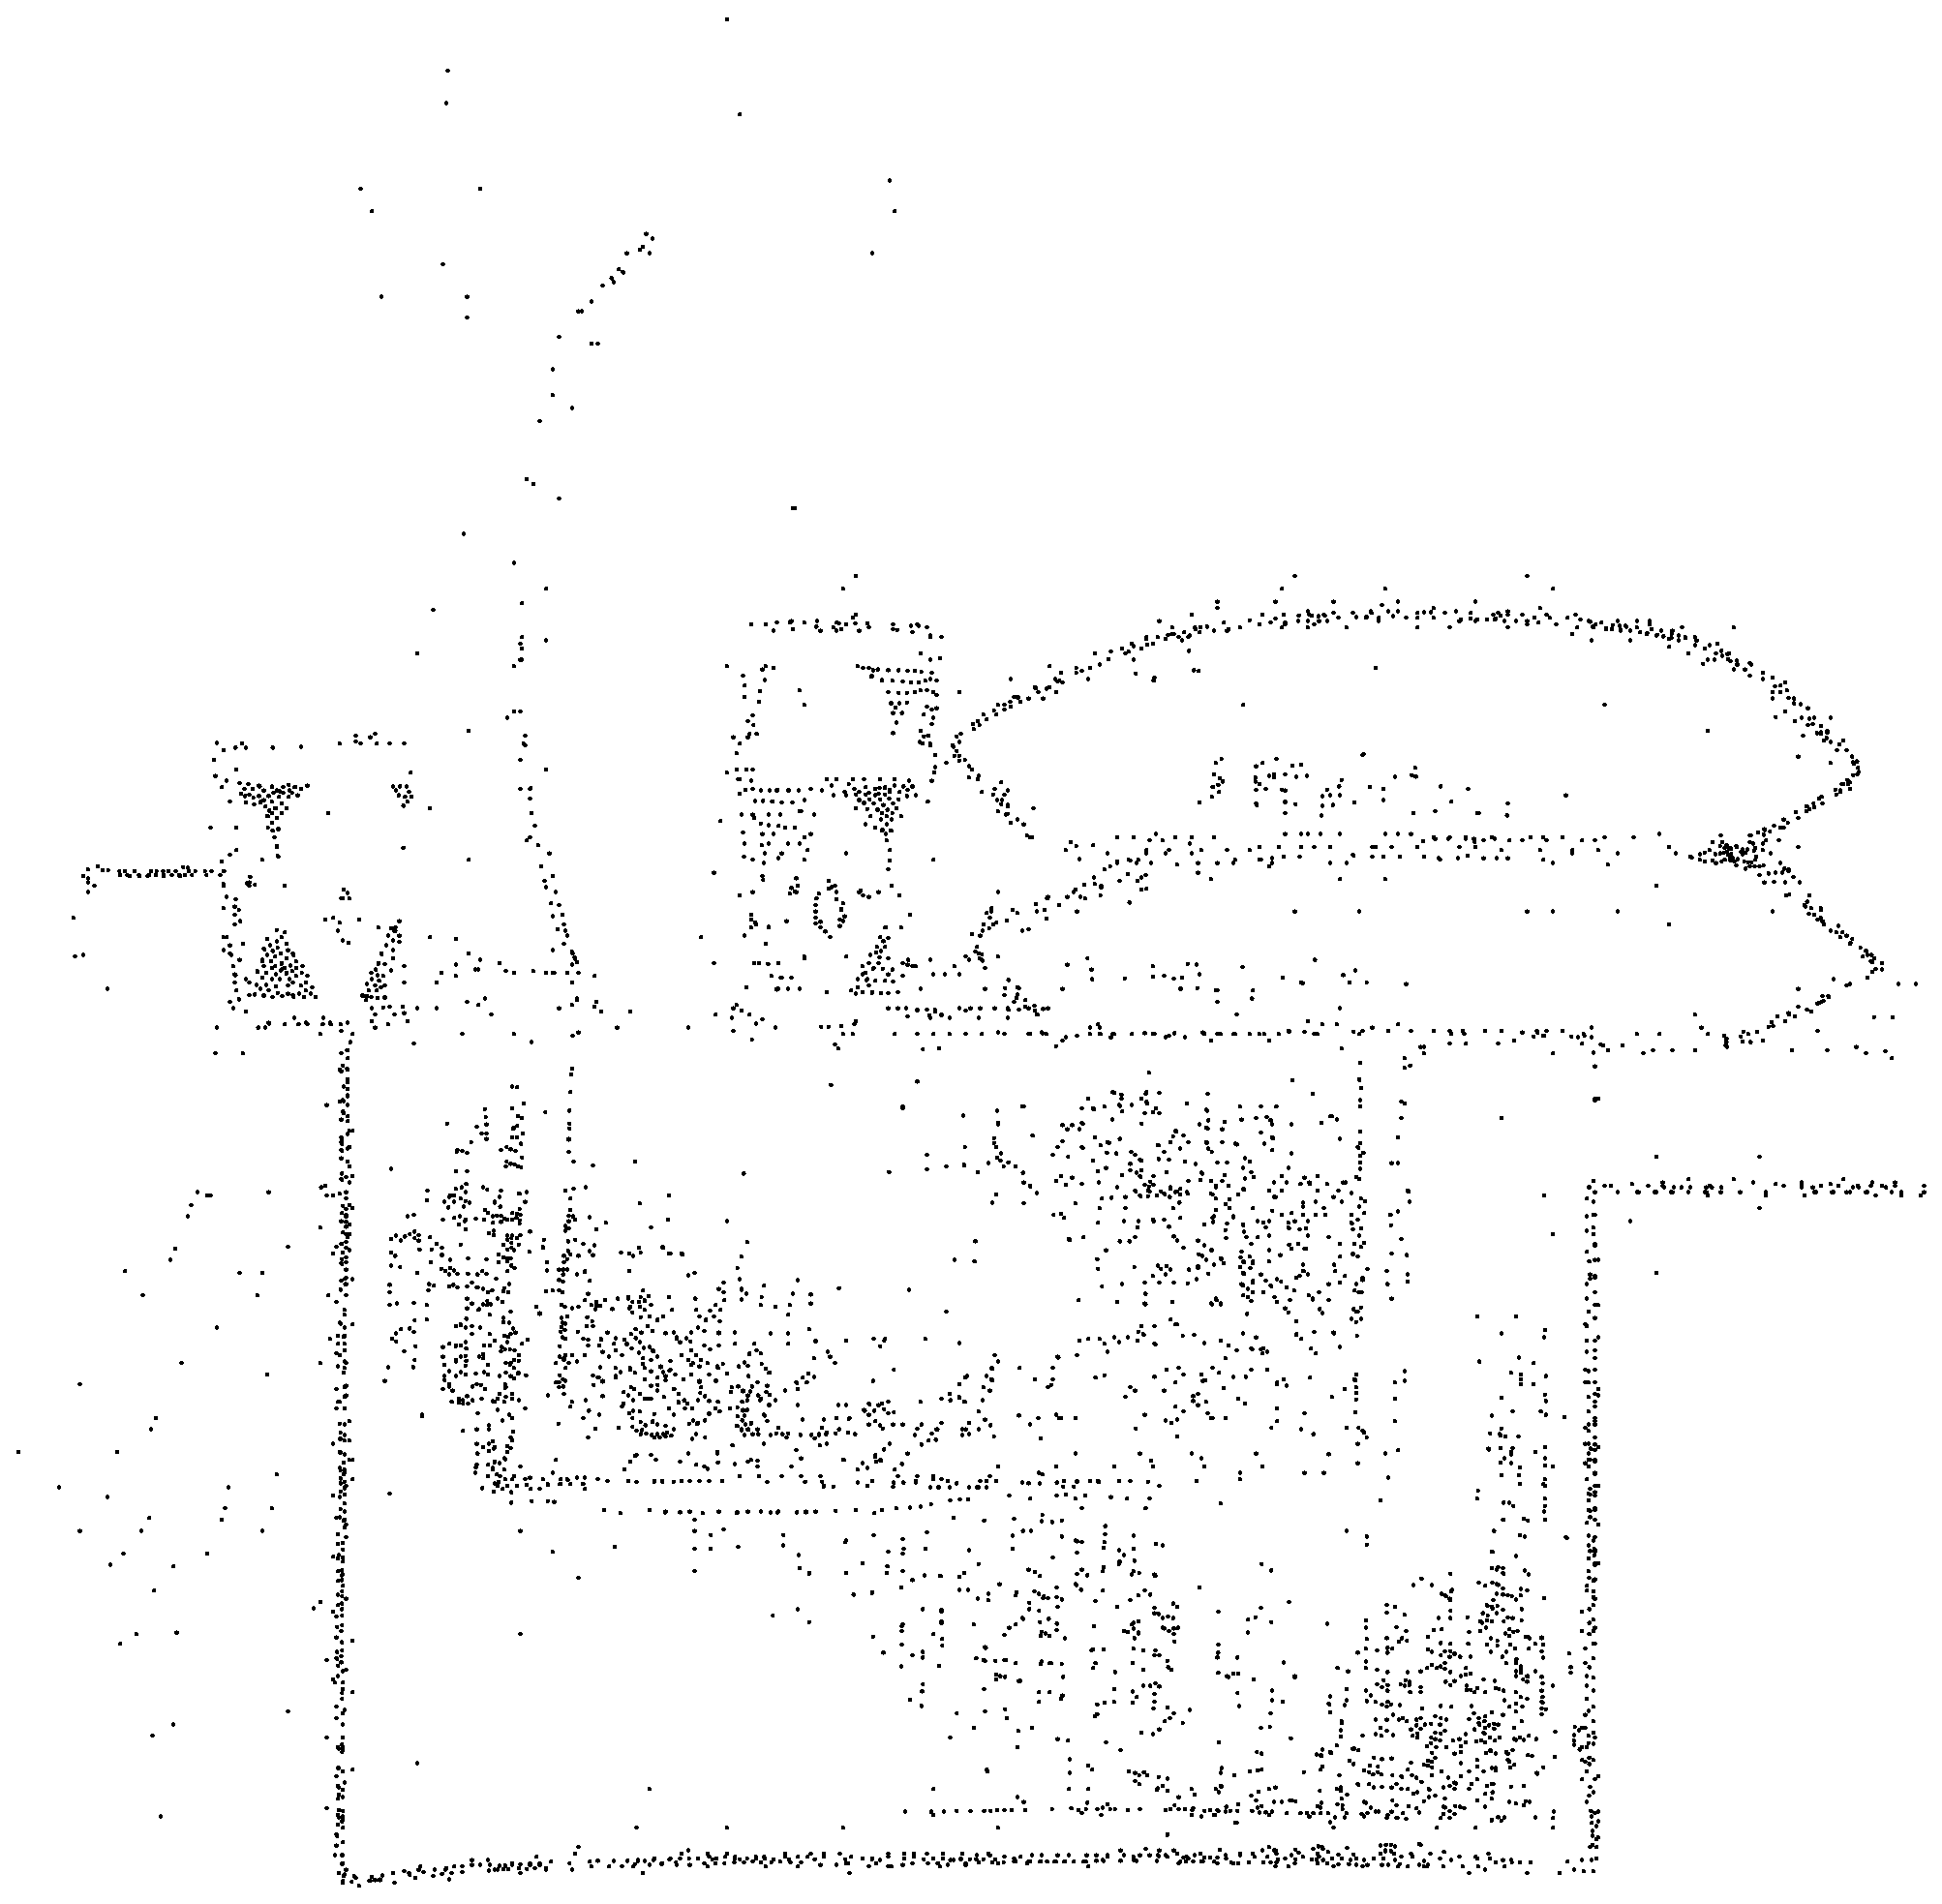
\includegraphics[width=0.45\textwidth]{1Extrema} }
  \caption{Titel der Grafik}
  \label{Bild1}
\end{figure}

\section{Keypoint-Reduktion und Verschiebung auf Subpixel-Ebene}
Dazu gehört Bild \ref{Bild2}.

\begin{figure}[htbp]
  \centering
  \includegraphics[width=0.45\textwidth]{2SubpixelmHintergrund} 
  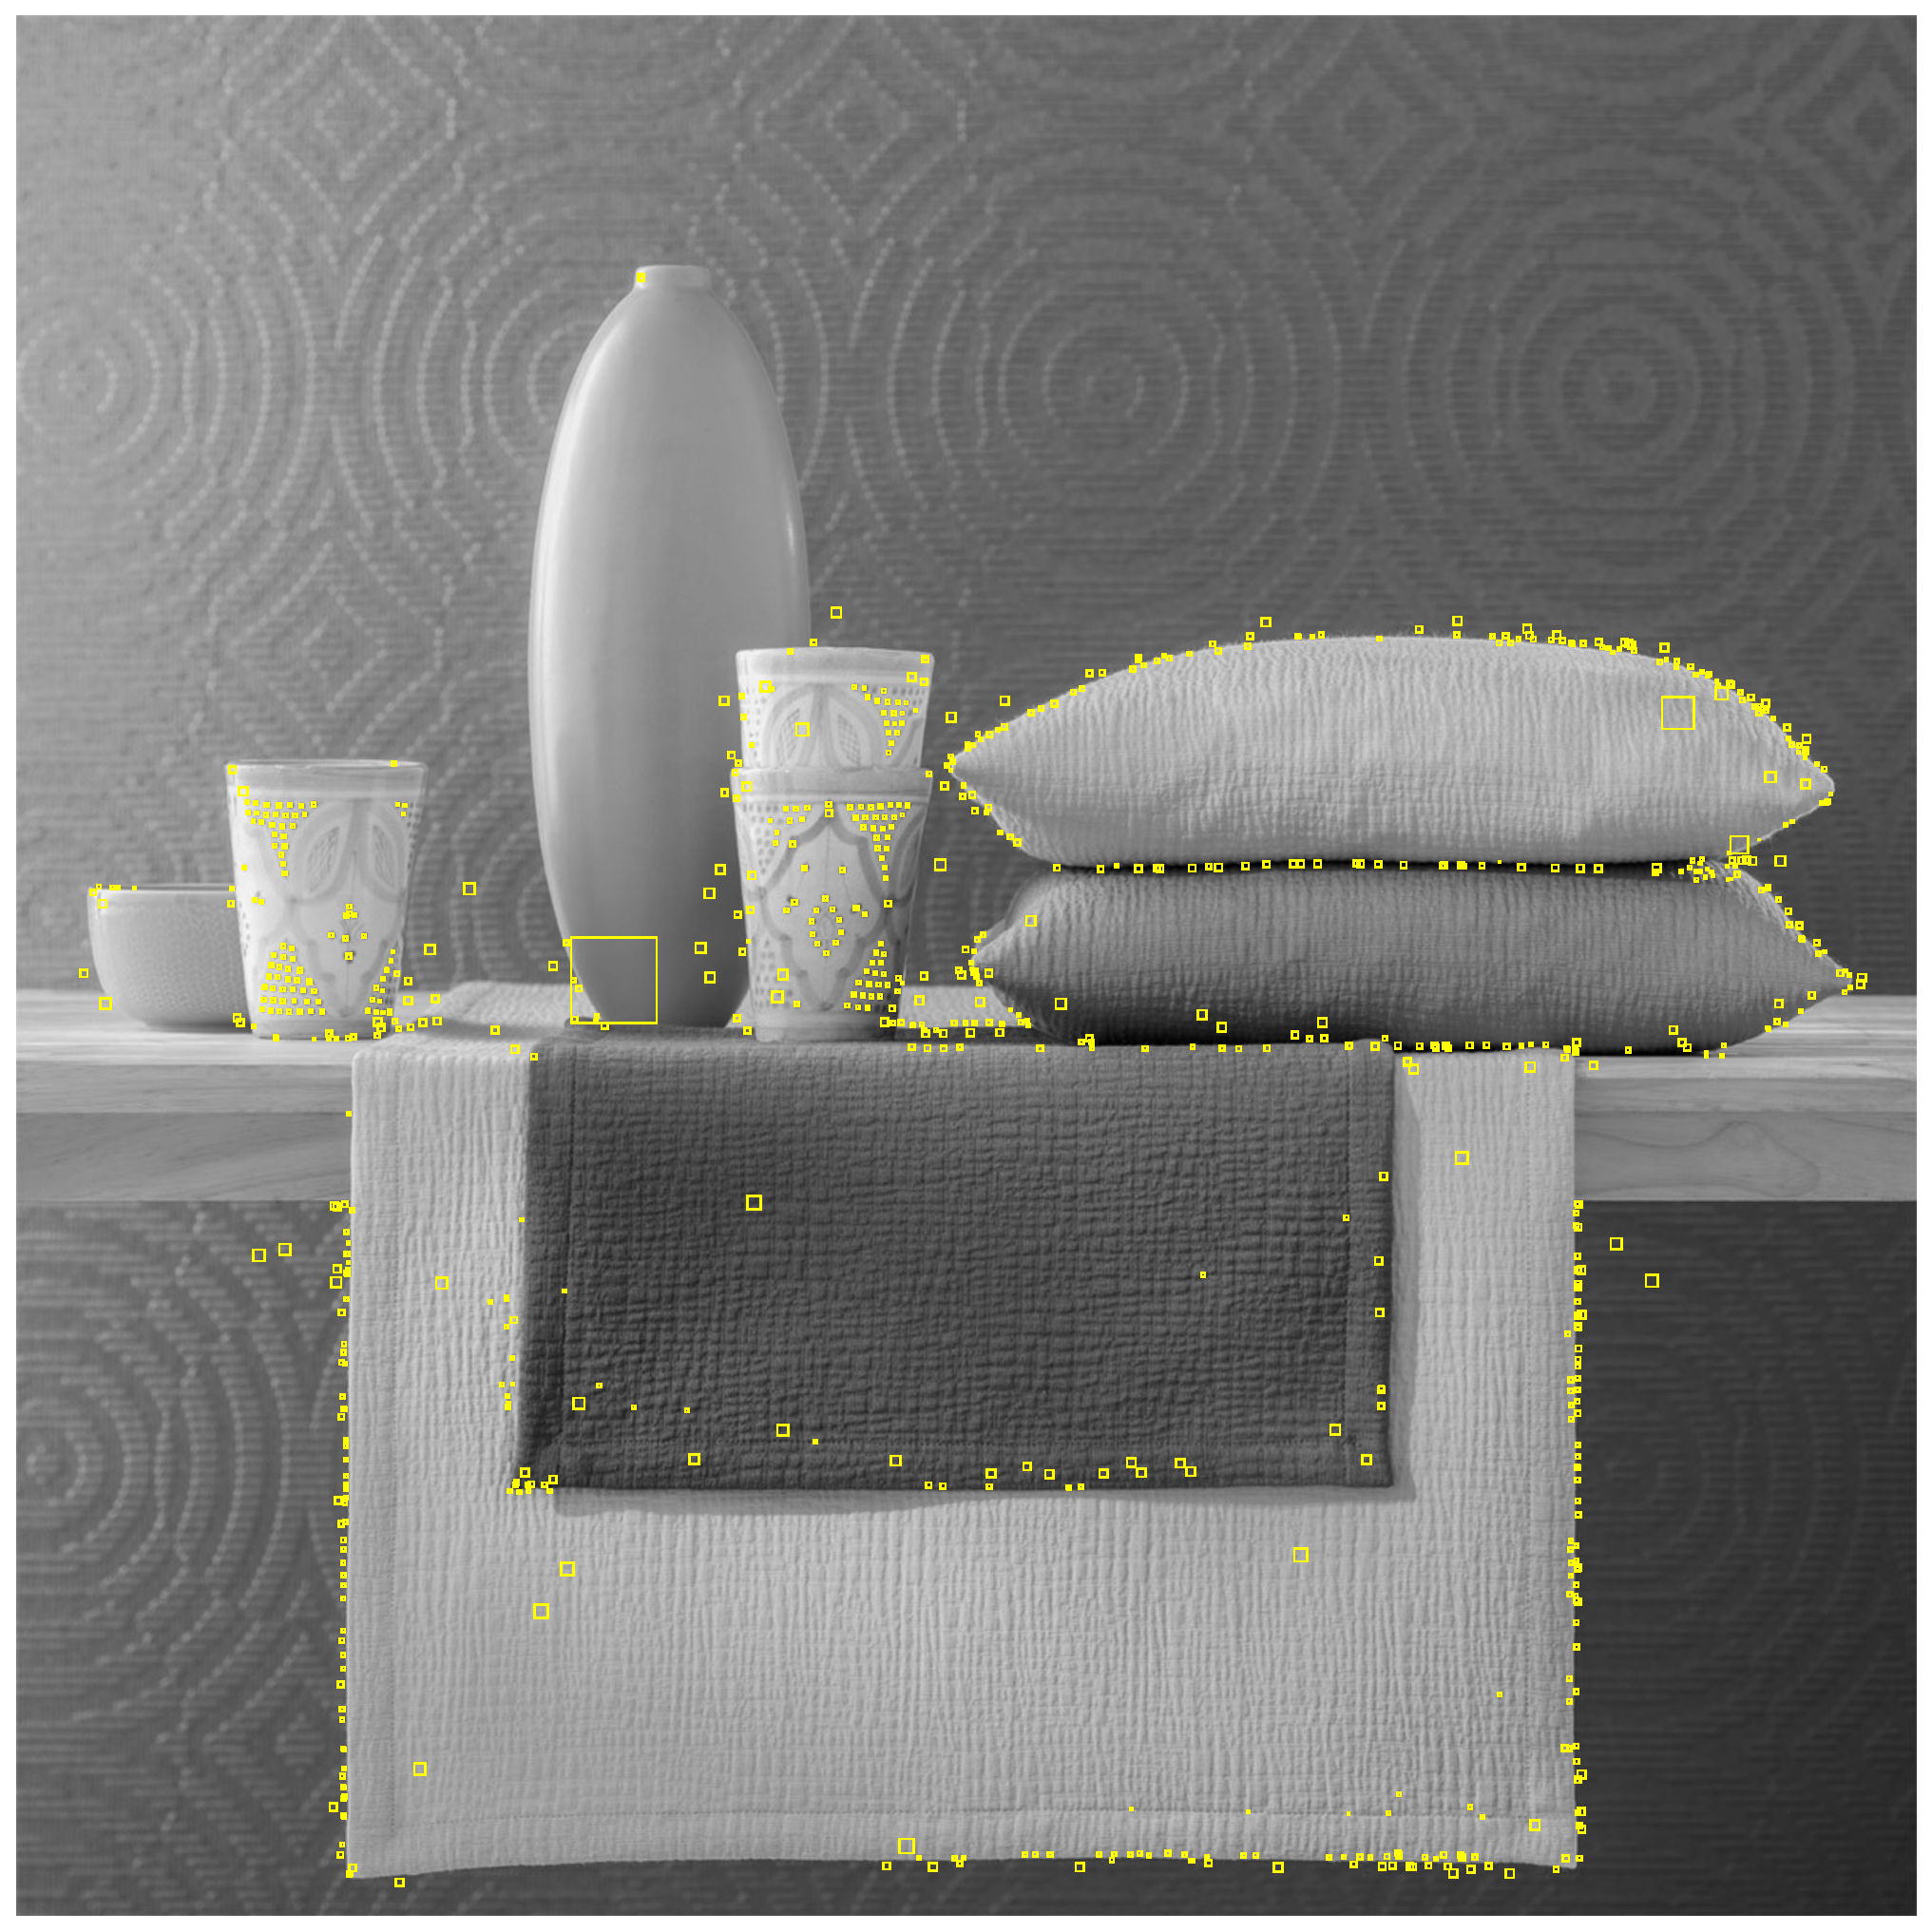
\includegraphics[width=0.45\textwidth]{4RechteckemHkorrigiert} 
  \includegraphics[width=0.45\textwidth]{5RechteckOrientierung} 
  \includegraphics[width=0.45\textwidth]{6RechteckOrientierungLastVer} 
  \caption{Titel der Grafik}
  \label{Bild2}
\end{figure}

\section{Keypoint-Orientierung}

\section{Keypoint Deskriptoren}

\section{Vergleich des Erreichten mit der Vorgabe}

%%%% Literatur
\newpage
\begin{thebibliography}{------}
\bibitem[Lowe04]{Lowe}
  David G. Lowe: {\em Distinctive Image Features from Scale-Invariant Keypoints}. 
  International Journal of Computer Vision 60(2): pp 91-110 (2004)
\end{thebibliography}

\end{document}          
